\section{Umsetzung}\label{kap:ums}
   
\subsection{C++ Library LibPiFace}
Wie im vorhergenenden Abschnitt *REF* beschrieben, bildet die Erweiterungskarte PiFace Digital 2 *REF* die Grundlage für diese Bachelorarbeit. Im Lieferumfang befindet sich eine in C geschriebene Library inklusive eines Lauffähigen Tests, welche ebenfalls auf GitHub unter https://github.com/piface/libpifacedigital zu finden ist. Diese Library stützt sich wiederrum auf die Library https://github.com/piface/libmcp23s17 welche den verbauten SoC über SPI anspricht. Im Laufe der Arbeiten fiel jedoch auf, dass die C Library nicht alle benötigten Funktionen enthielt. Da der Quellcode vorlag, und die Lizensierung Veränderungen am Quellcode zulässt, lag die Überlegung nahe die benötigten Funktionen direkt in der Library zu ergänzen anstatt sie im eigentlichen Projekt unterzubringen. Weiterhin schien es auch ein erstrebenswertes Lernziel zu sein, das Erstellen und Übersetzen von statisch bzw. dynamisch gelinkten Bibliotheken kennenzulernen. Zuletzt schien es schlichtweg die Sauberste Lösung zu sein. Zunächst wurde angenommen, dass sich auch mehrere Hardwaremodule per SPI mit einem einzelnen Rasperry Pi verbinden lassen. Dies ist technisch auch möglich, so bieten die eingesetzten Boards die Möglichkeit über einen Jumper eine Hardwareadresse einzustellen. Der Hersteller bot auch die passende Hardware an, um mehrere Boards mit einem Rasperry Pi zu verbinden. Jedoch wurden diese scheinbar mangels Nachfrage aus dem Sortiment genommen. Obwohl eine Bastellösung es immer noch ermöglichen würde, ist der Aufwand hierfür sehr hoch und scheint unwirtschaftlich. Leider wurde bis zu dieser Erkentniss schon einiges an Energie darin investiert, mehrere Boards zu unterstüzen. Dies ist auch der Grund wieso ein Objektorientierter Ansatz in C++ gewählt wurde - eine Instanz für jedes Harwaremodul. Ein weiterer Grund war, dass die Anwendung ohne Caching nicht performant genug war. Das heißt die zeitliche Lücke zwischen einer Änderung an einem Eingang bis zu dessen Auswirkung am Ausgang war deutlich spürbar. Dafür wurden Methoden vorgesehen, um das Caching ein un auszuschalten - bei eingeschaltetem Caching verändern die Methoden um Bytes und Bits zu schreiben, lediglich den Wert einer Instanzvariable. Derzeit muss das leeren des Chaces explizit mittels Aufruf der Methode \textit{flush()} erfolgen. Über ein Automatisches verfahren wurde nachgedacht, jedoch erwies sich der manuelle Aufruf als einfacher. 

\subsection{Parsen von Logikausdrücken}
Das Ziel dieses Projektes ist es, dass die Ausgänge der Steuerung in Abhängigkeit von Eingängen wie physikalischen Eigängen oder zum Beispiel Timer-bausteinen ein beziehungsweise ausgeschaltet werden. Dafür ist in einer Textdatei für jeden Ausgang eine Zeile vorgesehen. Eine Zeile beginnt hierbei mit dem zu definierenden Ausgang, also zum Beispiel Ho1, worauf ein Gleichheitszeichen zu folgen hat. Der gesamte Ausdruck hinter dem Gleichheitszeichen wird zur Laufzeit des Programms durchlaufen, wobei jedes vorkommende Paar von [ und ] durch eine Null oder eine Eins ersetzt. Innerhalb der Klammern, findet sich gleich genau wie bei dem Bezeichner vor dem Gleichheitszeichen, die jeweilige Bezeichnung der Abhängigkeit. Lautet die Zeile also etwa Ho0= [Hi0] \& [Hi1] so wird die Komplette erste Klammer durch den Wert von Hi0 ersetzt, wärend die zweite Klammer  durch den Wert von Hi1 ersetzt wird. Daraus ergibt sich dann, vorausgesetzt Hi0 und Hi1 sind im Zustand \chphl{Ein}, Ho0= 1 \& 1. Das für den Leser offensichtliche Ergebnis dieser Gleichung ist 1 oder \chphl{true}. Jedoch gestaltet sich eine programmatische Lösung des Problems als deutlich komplexer. Denn sobald mehr als drei Ausdrücke im Spiel sind, müssen wie bei klassischer Mathematik Rechenregeln befolgt werden. Punkt vor Strich sowie die Beachtung von Klammern. Dabei kann ein Ausdruck beliebig Komplex sein. Eine Rechersche nach Ansätzen führte zu Stackoverflow. (Siehe  
\footnote{Abr. 11.03.2019 \url{https://stackoverflow.com/questions/8706356/boolean-expression-grammar-parser-in-c/8707598\#8707598}}
 und  \footnote{Abr. 11.03.2019 \url{http://coliru.stacked-crooked.com/a/c40382620fb75b75}}) Dieser Ansatz löste genau das Problem und wurde somit in das Projekt übernommen. 
%
\subsection{Automatische Prüfung von Abhängigkeiten}
Ein Problem was sich mit dem Einbinden der Lösung zum Parsen der Logikausdrücke ergab, war die Abhängigkeit zu Boost. Auf dem Desktop Computer auf dem die Lösung getestet wurde, konnte das Projekt dank installiertem boost Paket ohne Probleme übersetetzt werden. Da es sich bei dem  Zielsystem jedoch um eine ARM Architektur handelt, musste der code dort Übersetzt werden. In den Paketquellen des dort installieren Raspian, ist jedoch eine ältere Version des Boost Pakets hinterlegt, was dazu führt dass Boost manuell heruntergeladen und gebaut werden muss. Obwohl sich dieses Problem im Laufe der Zeit durch aktualisierung des Paketes in den Paketquellen von Raspian von selbst lösen wird, muss dennoch geprüft werden ob die installierte Version den Ansprüchen genügt. Hierfür wurde ein Bash script erstellt, welches auch alle weiteren abhängigkeiten Prüft und gegebenenfalls installiert. Dazu zählen auch die in *REF* erwähnten Bibliotheken um die Hardware anzusprechen und wie in *REF* erwähnt der verwendete Kompiler. 
 
\subsection{Benamungsschnema}
Nachdem die Auswertung beziehungsweise das Parsing der Logikausdrücke funktionierte, sollte auch die Auswertung der Bezeichner automatisiert werden. Ein Benamsungsschema wurde dabei schon vorher erdacht. Es besteht aus einem führenden Großbuchstaben, gefolgt von einem Kleinbuchstaben und einer Zahl. Dabei wird der führende Buchstabe als Kanal bezeichnet, der zweite als Entität und die Ziffer als Pin-Nummer. So könnte zum Beispiel der Buchstabe \chphl{H} den Kanal Hardware beschreiben, welcher  wiederrum die Entitäten \chphl{i} für Input und \chphl{o} besitzt, welche jeweils ein Byte, also 8 Bits oder Pins haben. 

\subsection{Klassenstrukrur und Kanäle}
Im Programm werden die zuvor beschriebenen Kanäle von einem Abkömmling der Basisklasse \chphl{IO\_Channel} (siehe Abb. \ref{img:classIOChannel}) repräsentiert. Wobei jeder Kanal als Eigenschaft eine Map mit Entitäten führt, welche durch Objekte des Typs \chphl{Channel\_Entity} (siehe Abb. \ref{img:classChannelEntity}) repräsentiert werden. Eine Entität wiederum weiß, wie groß ihre Breite ist, also wie viele Bits sie hat und ob sie nur lesbar oder auch beschreibbar ist. Eine weitere Klasse \chphl{IO\_Channel\_AccessWrapper} (siehe Abb. \ref{img:classAgregation}) bündelt alle vorhandenen Kanäle inklusive der jeweiligen Entitäten. Zudem erleichtert Sie mittels Überladung der Array-Operatoren den Zugriff. Ein Zugriff ist dann wie in Listing \ref{code:chnlAccess} gezeigt wird möglich. Dazu müssen die Entsprechenden Kanäle vorher wie in Listing \ref{code:chlnInit} zu sehen initialisiert und einer Instanz der Klasse \chphl{IO\_Channel\_AccessWrapper} übergeben werden. Der für den späteren Zugriff auf den Kanal nötige Buchstabe, wird in diesem Zuge festgelegt, während die Buchstaben der untergeordneten Entitäten Bestandteil des jeweiligen Kanals sind und dementsprechend dort definiert werden. 


\begin{listing}[H]
	\inputminted[numbersep=1pt,fontsize=\scriptsize,frame=single, firstline=364,lastline=369]{c}{./code/main-klassenstruktur.cpp}
	\caption{Initialisieren der Kanäle und Entitäten}
	\label{code:chlnInit}
\end{listing}


\begin{listing}[H]
	\inputminted[numbersep=1pt,fontsize=\scriptsize,frame=single, firstline=415,lastline=416]{c}{./code/main-klassenstruktur.cpp}
	\caption{Zugriff auf Kanal und Entität exemplarisch}
	\label{code:chnlAccess}
\end{listing}


\begin{figure}[H]
	\begin{center}
		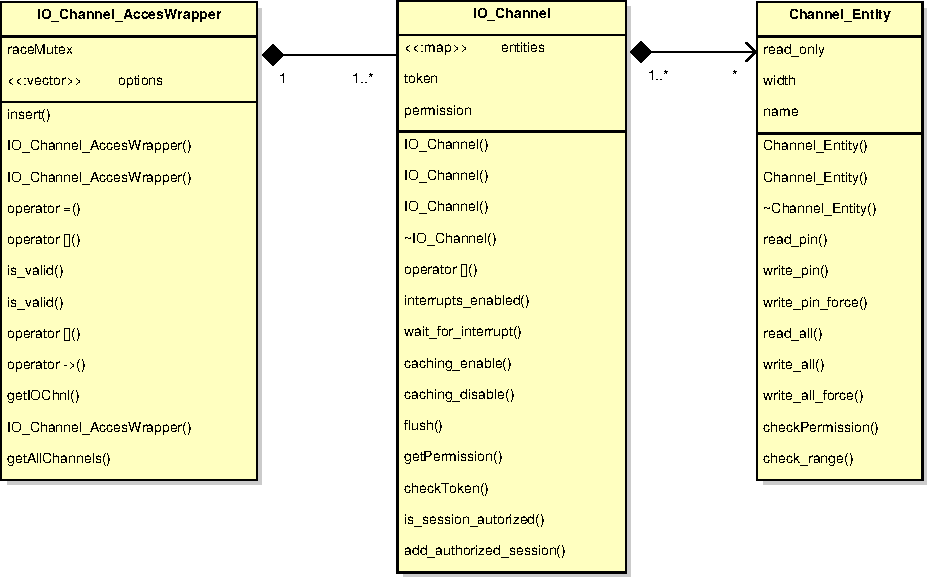
\includegraphics[width=0.95\textwidth ,clip]{./code/Aggregation.pdf}
		\caption{Klassendiagramm Aggregation der Klassen}
		\label{img:classAgregation}
	\end{center} 
\end{figure}	
Zu sehen ist die Aggregation zwischen dem \chphl{IO\_Channel\_AccessWrapper} den Kanälen \chphl{IO\_Channel} und den Entitäten \chphl{Channel\_Entity}. Alle Kanäle werden von dem  \chphl{IO\_Channel\_AccessWrapper} zusammengefasst. Ein Zugriff erfolgt ausschließlich über diesen Weg. 


\begin{figure}[H]
	\begin{center}
		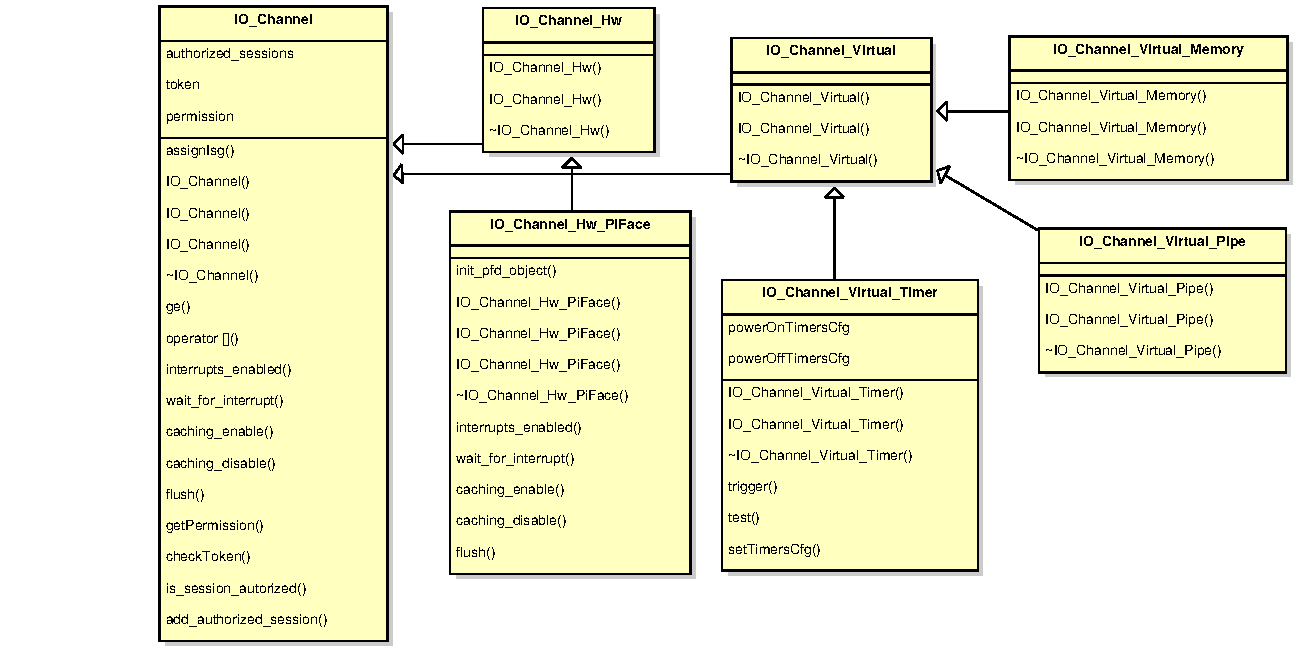
\includegraphics[width=0.95\textwidth ,clip]{./code/IOChannel.pdf}
		\caption{Vererbungshierarchie der Basisklasse IOChannel}
		\label{img:classIOChannel}
	\end{center} 
\end{figure}	

\begin{figure}[H]
	\begin{center}
		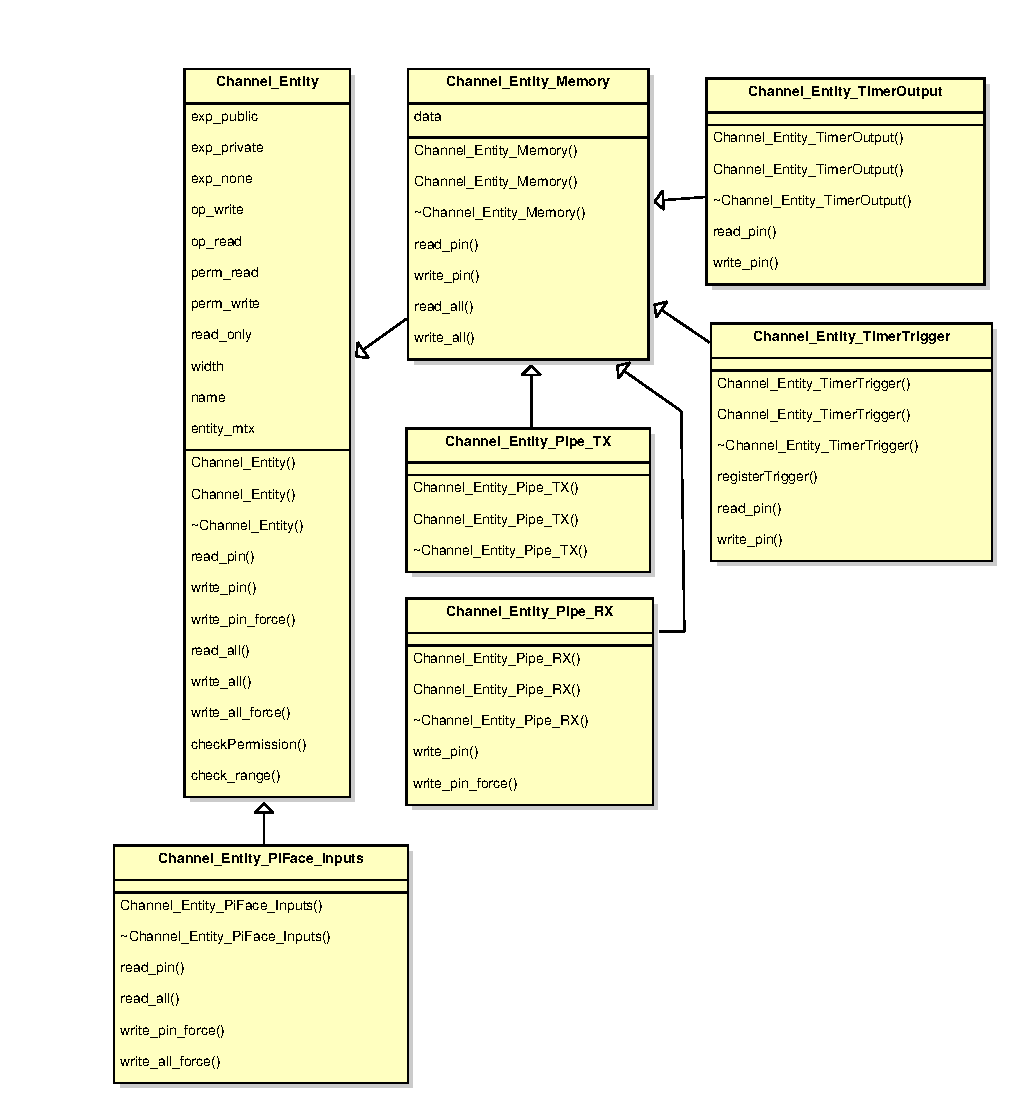
\includegraphics[width=0.95\textwidth ,clip]{./code/ChannelEntity.pdf}
		\caption{Vererbungshierarchie der Basisklasse ChannelEntity}
		\label{img:classChannelEntity}
	\end{center} 
\end{figure}	

Die Entitäten erben von der Basisklasse Entity. Sie überschreiben Methoden um lesend oder schreibend, entweder auf den gesamten Inhalt auf einmal oder Bitweise auf den Inhalt zuzugreifen. Dafür sind die Methoden read\_pin, write\_pin beziehungsweise read\_all und write\_all vorgesehen. 



\subsubsection{Hardware Kanäle}
Der Wohl wichtigste Kanal ist der Hardware Kanal. Die Klassenstruktur in Abb. \ref{img:classIOChannel} zeigt, dass alle Kanäle eine gemeinsame Basisklasse haben. Der Hardware Kanal ist eine Spezialisierung der Basisklasse, welche spezifische Funktionen für die Entsprechende Hardware beherbergt. So finden sich hier Methoden zur Steuerung des Caching sowie ein blockierender Aufruf, welcher auf einen Interrput an der Hardware reagiert. Die Funktionen für den schreibenden und lesenden Zugriff auf die Ein- und Ausgänge der Hardware, sind in Entitäten gekapselt. Für eben jenen Zweck existieren zwei Spezialisierungen der \chphl{Channel\_Entity} (siehe Abb. \ref{img:classChannelEntity}) Basisklasse, welche für den Zugriff mit \chphl{i} für den Eingang (input) beziehungsweise \chphl{o} für den Ausgang (output) referenziert werden.   

\subsubsection{Merker Bausteine}
Die erste Erweiterung, welche wie in Abb. \ref{code:chlnInit} zu sehen mit dem Buchstaben M referenziert wird, sind Memory Bausteine. Da ein Memory Baustein nicht richtungsorientiert sind, das heißt es existiert keine Eingangs oder Ausgangsgröße, wurde hier vom Benamsungsschema für Entitäten  abgewichen. Eine Referenzierung ist hier mittels eines oder mehrerer Buchstaben geplant. Somit bietet ein Merker Baustein Platz für 8 Zustandswerte pro verwendeter Entität. Bislang ist lediglich die Entität \chphl{a} angelegt, wobei geplant ist die Anzahl an Buchstaben beziehungsweise Entitäten durch einen Konstruktorparameter nach Außen zu führen, womit die Anzahl wie in Abb. \ref{code:chlnInit} zu sehen beim Einfügen bestimmt werden könnte, oder in einem weiteren Schritt in eine Konfigurationsdatei exportiert werden kann. 

\subsubsection{Timer Bausteine}
Timer Bausteine waren die wohl komplexesten Bausteine. Eine Verzögerung im Programmablauf bedeutet entweder ein blockieren, was aber bedeuten würde, dass das Programm in dieser Zeit auch nichts anderes tun kann und somit nicht auf Ereignisse reagieren kann. Die andere alternative ist Multithreading, also das Einführen von Parallelen Handlungssträngen, welche weitere Probleme bringen. So muss zum Beispiel beim Zugriff auf gemeinsam genutzte Ressourcen dafür sorge getragen werden, dass nicht gelesen wird während gerade geschrieben wird. Des weiteren musste die Hauptschleife überarbeitet werden. Bislang wurde die Programmlogik bei jedem eintreten eines Hardware-Ereignisses genau einmal durchlaufen. Jedoch muss die Programmlogik nun auch durch Ablauf eines Timers erneut durchlaufen werden. Gelöst wurde dies mithilfe einer Binären Variable als Schalter, welche zusammen mit eines Mutex zur Vermeidung von gleichzeitigem Zugriff, und einer Condition Variable zur Benachrichtigung des Hauptprozesses, in die Klasse \chphl{iterationSwitchGuard} gekapselt wurde. 
Ein Timerbaustein (mehrere sind Theoretisch möglich), bietet 8 Konfigurierbare Timer. Dabei gibts es eine Entität um einen Timer auszulösen \chphl{t} (Trigger) und eine Entität, welcher als Ausgang fungiert \chphl{o} (Output). So ergibt sich in der Programmlogik die selbe Syntax, welche sich auch bei Hardwarekanälen bietet: Ein explarisches triggern des Timers 3 würde erfolgen, indem eine Zeile der Logikdatei mit \chphl{Tt3=} beginnt. Eine Verwendung des Ausgangswertes desselben Timers, würde durch integrieren des Bezeichners \chphl{[To3]} in die Logikzuweisung eines anderen Bezeichners erfolgen. Die Parametrisierung des Timers erfolgt durch einbinden einer Konfigurationsdatei (siehe Listing \ref{code:timersConf}) hierbei lassen sich für jeden Timer eine Einschaltverzögerung sowie eine Ausschaltverzögerung definiert werden. Jeder Wert ungleich null bewirkt eine Verzögerung, eine gleichzeitige Nutzung von Ein und Ausschaltverzögerung ist möglich. Werte gleich null bewirken eine sofortige Änderung am Ausgang, sobald sich der Eingangswert verändert. Beim Einlesen der Konfiguarionsdatei werden sämtliche Leerzeichen entfernt. Zudem kann mit einem Semikolon \chphl{;} oder einer Raute \chphl{\#} ein Kommentar eingeleitet werden, welches alle restlichen Zeichen der Zeile beim Einlesen entfernt. Die Verzögerungszeiten sind in Millisekunden anzugeben, wobei die Reihenfolge der nicht sukzessive erfolgen muss. Der Maximalwert beläuft sich auf 4.294.967.295, was die größte in unsignes long darstellbare Zahl ist und umgerechnet etwa 49 Tagen entspricht. 
\begin{listing}[H]
	\inputminted[numbersep=1pt,fontsize=\scriptsize,frame=single, firstline=14,lastline=25]{c}{./code/timers.conf}
	\caption{Beispiel der Timer Konfigurationsdatei}
	\label{code:timersConf}
\end{listing}


\subsubsection{Virtuelle Kanäle}
Virtuelle Kanäle sind ein Konzept dass die Kommunikation der Steuerung mit entfernten Endpunkten ermöglichen. Ein Virtueller Kanal ist hierbei lediglich ein veränderter Memory Baustein, welcher entgegen entgegen anders als ein normaler Memory Baustein wieder richtungsorientiert ist. Das heißt es gibt eine Eingangs-Entität und eine Ausgangs-Entität. Hierbei muss beachtet werden, dass die Perspektive so gesetzt ist, dass ein Eingang die extern empfangenen Daten beinhaltet. Während in den Ausgang geschrieben wird. Die Gegenseite bildet der in *REF* beschriebene WebSocket Server, beziehungsweise was auch immer die Gegenseite bildet. Das kann das WebFrontend *REF* dieses Projektes sein, oder auch jeder andere WebSocket fähige Client. Angedacht ist auch die Implementierung eines WebSocket Clients in das Backend, womit sich zwei Einheiten verbinden ließen. 


\subsection{Laden der Programmlogik aus Datei}
Das Logikprogramm wurde im nächsten Schritt in eine Textdatei ausgelagert. Sie soll künftig von der grafischen Benutzeroberfläche automatisch erstellt werden können, kann aber nach wie vor auch von Hand erstellt werden. Die Datei enthält einen Ausgang pro Zeile, gefolgt von einem Gleichheitszeichen und den Abhängigkeiten. Zeichen die auf ein Semikolon folgen, werden dabei als Kommentar gewertet und ausgelassen. Sie wird bei Programmstart eingelesen und verbleibt dann im Speicher.  

\begin{listing}[H]
	\inputminted[numbersep=1pt,fontsize=\scriptsize,frame=single, firstline=29,lastline=36]{c}{./code/logic.conf}
	\caption{Beispiel der Programmlogik Datei}
	\label{code:c}
\end{listing}


\subsubsection{Erneutes Laden der Logik zur Laufzeit}
Zum erneuten einlesen der Logik, wurde ein Signalhandler vorgesehen, welcher auf das Signal SIGUSR1 hört. Die entsprechende Funktion ließt dann die Logikdaten erneut ein und überschreibt damit die vorherige Version im Speicher. Damit muss die Steuerung nicht neu gestartet werden und ermöglicht das Steuerungsprogramm zur Laufzeit zu verändern.


\subsection{Hauptschleife und Iterationslogik}
Das Logikprogramm liegt nun im Speicher und das Programm betritt die Hauptschleife. Doch treibt ein einfaches polling die Auslastung des Prozessors unnötig nach oben. Nun könnte nach jedem Durchlauf eine gewisse Zeit gewartet werden, bevor eine neue beginnt. Doch das verringert die Reaktionszeit der Steuerung. Die beste Lösung findet sich direkt im Treiber des PiFaceDigital. Hier bietet sich eine Funktion, die bis zum Eintreten einer Veränderung der  Eingangswerte blockiert. Intern Eingesetzt wird hier ein Epoll, welcher einen File descriptor auf einen der GPIOs des Raspberry Pi überwacht und diesen somit als Interrupt Kanal nutzt. 


Beschreibung, Begründung
 
\clearpage
